\section{Einleitung}%2-10

Diese Studienarbeit dokumentiert den Programmentwurf einer Party-Lichtsteuerung vom Design der Anwendung über die Implementierung bis hin zur Bereitstellung einer lauffähigen Applikation.
Die Programmcode wird mit LabVIEW von National Instruments entwickelt.

\subsection{Aufgabenstellung}
Es ist ein Programm für Lichttechniker zu entwickeln, mit dem eine Vielzahl von Scheinwerfern angesteuert werden kann. 
%Dabei soll ein durch den Lichttechniker erstellter Ablauf abgespielt werden.

\subsection{Anforderungen}
Der Light Jockey (LJ) stellt für verschiedene Lichtkanäle Intensität und Farbe ein. 
Für eine Gruppe von Lichtkanälen (Set) kann eine Wartezeit, Überblendungszeit, Nachlaufzeit und ein Name eingestellt werden. 
Wählt der LJ die Schaltfläche zum Aufnehmen, öffnet sich ein Fenster, in dem die gewünschten Parameter übergeben werden. 
Nach der Bestätigung durch einen Klick auf die OK-Schaltfläche wird das erstellte Set an das Ende einer wählbaren Queue angefügt.

Hat der Bediener einige Sets angelegt und zu einer Queue zusammengefügt, wird mit der Abspiel-Schaltfläche das aufgenommene Programm durchlaufen. 
Ein Set, das abgespielt wird wartet die angegebene Zeit, dann wird die Farbe bis zur Intensität über die Überblendungszeit hochgefahren. 
Danach beginnt die Nachlaufzeit.
Ist diese verstrichen, wird mit dem nächsten Set aus der Queue fortgefahren. 
Der Bediener kann jeder Zeit eine abspielende Queue mit der Stopp-Schaltfläche anhalten.

Über die Menüleiste kann der Bediener mit dem Menüpunkt "`Datei"' die Queue speichern und laden. 
In beiden Fällen öffnet sich eine Dialogbox in der nach Speicher- bzw. Ladepfad gefragt wird.

	\begin{figure}%[h!]
	\centering
		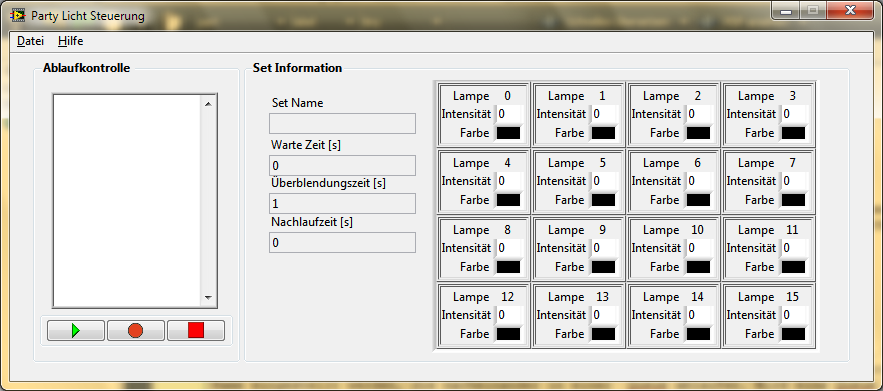
\includegraphics[width=\textwidth]{Pics/Oberflaeche001.png}
	\caption{Bedienoberfläche für die Party-Lichtsteuerung}
	\label{fig:ober001}
	\end{figure}



%\subsection{Motivation und Zielsetzung}

%Quelle: \cite{labview-buch01} \\
%Quelle: \cite{internet}
\subsection{Dokumentation}
Der LabVIEW Quellcode  sowie eine ausführbare Windows-Anwendung mit dem notwendigen RunTime-Installer befindet sich auf der beigelegten CD.
Ebenfalls enthalten sind Detailansichten der wesentlichen Programmcodeausschnitte.
%Und Projekt auf \url{http://code.google.com/p/party-licht-steuerung/}.


\subsection{Aufbau der Arbeit}

Zu Beginn wird auf LabVIEW als Programmiersprache eingegangen. Es werden verschiedene Entwurfsmuster für eine strukturierte Programmierung vorgestellt.
Darauf folgt die Programmanalyse mit der Datenabstraktion, einem Ablauf-  und einem Datenflussdiagramm. 
Im 4. Kapitel wird die Implementierung dokumentiert. 
Im darauffolgenden Kapitel wird ein spezieller Testfall beschrieben und ausgewertet. 
Ein Fazit und Ausblick auf Erweiterungen bilden den Abschluss. 
Im Anhang finden sich vergrößerte Codeausschnitte, sie wurden zur besseren Lesbarkeit aus dem Text ausgegliedert.




